\subsubsection{Jupyter Terminal}

\paragraph{Overview}


\bigskip
\centerline{\rule{13cm}{0.4pt}}
\bigskip

JupyterLab provides an an interactive shell in a terminal.

\begin{framed}
\textbf{Use the terminal to easily delete non-empty directories}\\
Jupyter intentionally prevents the deletion of non-empty directories from the file browser. However, you can delete full directories from the command line in a terminal.

\texttt{rm -rf path/to/my/full/directory}
\end{framed}

\paragraph{\textbf{How to Open a Terminal}}


\bigskip
\centerline{\rule{13cm}{0.4pt}}
\bigskip

\begin{enumerate}
\item If there is no \texttt{Launcher} tab in your workspace, open one by clicking the blue \texttt{+} button at the upper left of the screen.
\end{enumerate}

\begin{figure}[!htbp]
\centering
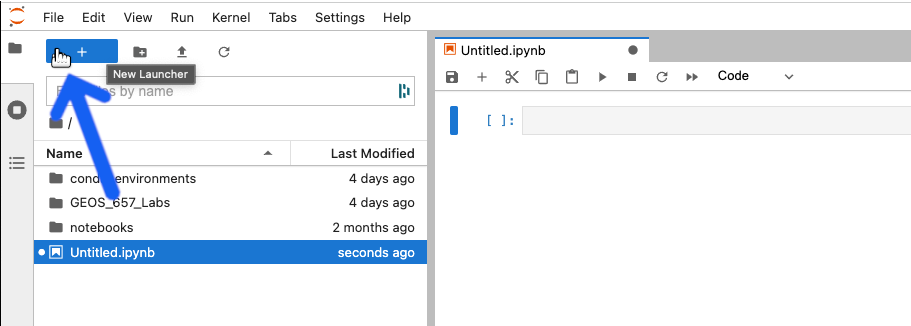
\includegraphics[width=0.7\linewidth]{files/launcher-c8502ccf02f11470216a123405d1af64.png}
\caption*{The JupyterLab \texttt{New Launcher} button}
\end{figure}

\begin{enumerate}[resume]
\item Click the \texttt{Terminal} button in the \texttt{Launcher} tab.
\end{enumerate}

\begin{figure}[!htbp]
\centering
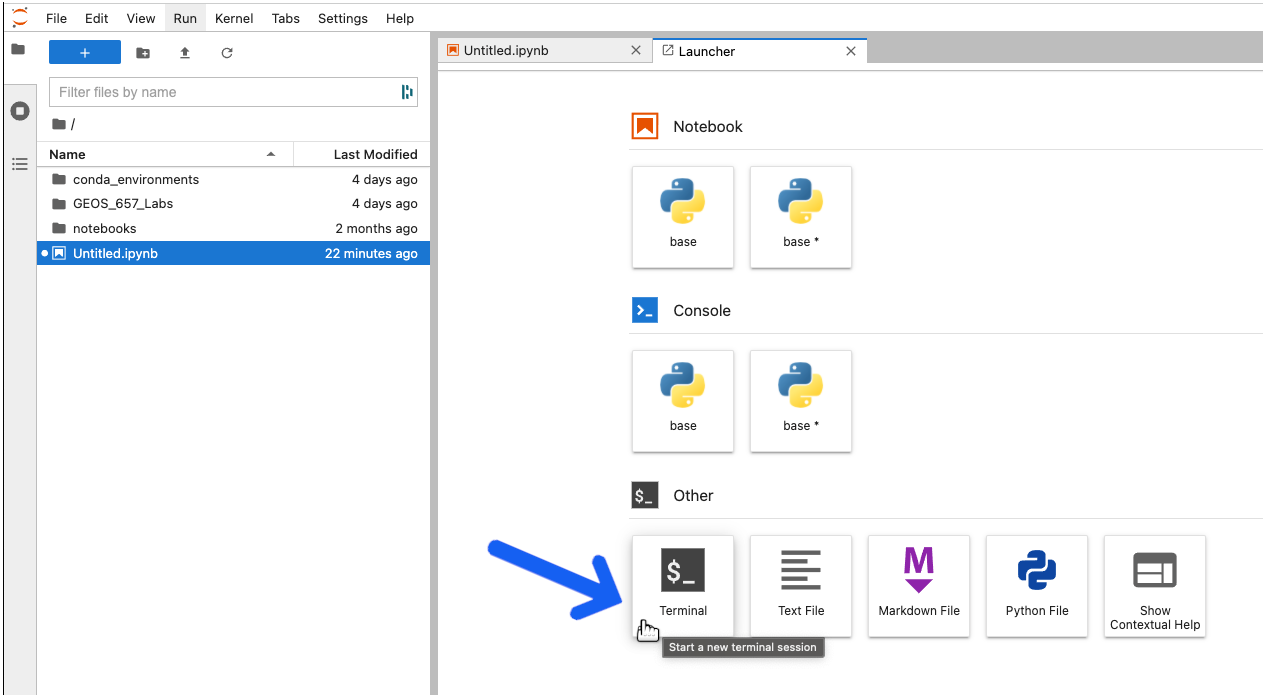
\includegraphics[width=0.7\linewidth]{files/jlab_terminal-f2d777f76897cfe77aa7041fd71d98ce.png}
\caption*{The JupyterLab \texttt{Terminal} button.}
\end{figure}

\begin{enumerate}[resume]
\item Use the terminal as you typically would.
\end{enumerate}

\begin{figure}[!htbp]
\centering
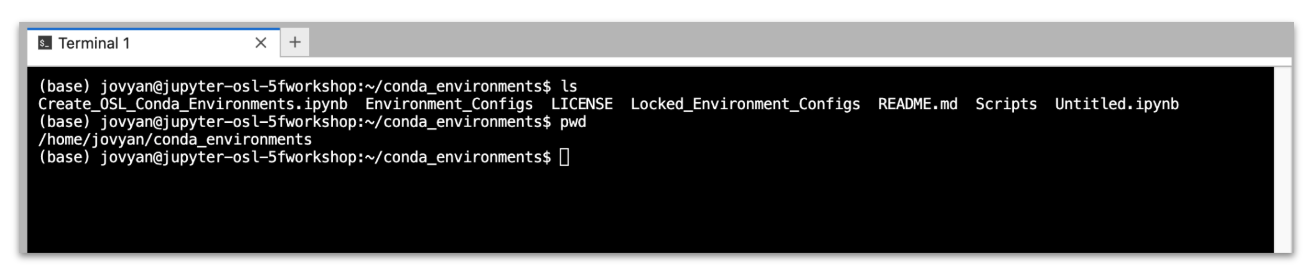
\includegraphics[width=0.7\linewidth]{files/terminal-9cc223d82afb11b942d56e6310abad5a.png}
\end{figure}


\bigskip
\centerline{\rule{13cm}{0.4pt}}
\bigskip

\begin{framed}
\textbf{No Root Privileges}\\
For security, OSL users do not have root privileges.

\begin{figure}[!htbp]
\centering
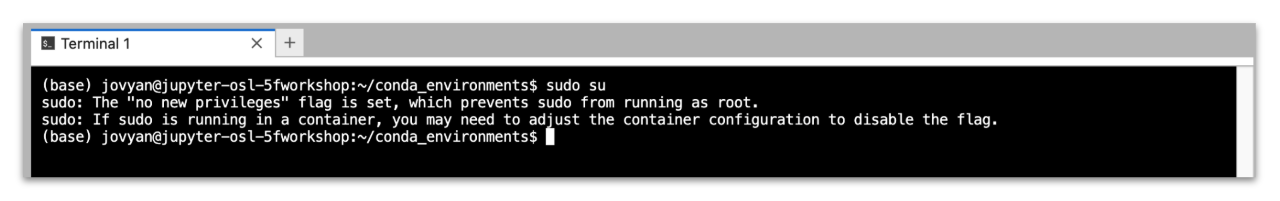
\includegraphics[width=0.7\linewidth]{files/no_sudo-d355e5fa49ab50be6c8011cc5806454e.png}
\end{figure}
\end{framed}